\newcommand{\mypathoj}{../thesis/oj}

\newcommand{\mypathojdata}{../thesis/oj/data}
%\newcommand{\scd}{\cD_\oplus}
%\newcommand{\btu}{\bigtriangleup}
\newcommand{\alert}[1]{#1}
%\newcommand{\mypathjcchere}{../thesis/jcc}
%\newcommand{\bE}{\mathbb{E}}
\newcommand{\bD}{\mathbb{D}}
\newcommand{\E}[2]{\mathbb{E}_{#1} \left[ #2 \right]}
\newcommand{\bP}[2]{\mathbb{P}_{#1} \left[ #2 \right]}
\newcommand{\dpO}{d\mathbb{P}_\Omega}
\newcommand{\feb}{f_e\left(\beta\right)}
\newcommand{\fenb}{f_{en}\left(\beta\right)}
\newcommand{\fehb}{f_e\left(\hat{\beta}\right)}
\newcommand{\pfeb}{\frac{\partial}{\partial \beta_j}\feb}
\newcommand{\pfenb}{\frac{\partial f_{en}\left(\beta \right)}{\partial \beta_j}}
\newcommand{\pfehb}{\frac{\partial f_e\left(\hat{\beta} \right)}{\partial \beta_j}}
\newcommand{\hye}{\hat{y}_e}
\newcommand{\hse}{\hat{s}_e}
\newcommand{\pe}{\pi_e}
\newcommand{\pn}{\pi_n}
\newcommand{\psen}{\psi_{en}}
\newcommand{\rand}{\boldsymbol{\delta}}
\newcommand{\ri}{\pmb{\delta^m}}
\newcommand{\rf}{\pmb{\delta^y}}
\newcommand{\rx}{\pmb{x}}
\newcommand{\rX}{\pmb{X}}
\newcommand{\rD}{\pmb{\Delta}}
\newcommand{\rdm}{\pmb{\delta^m}}
\newcommand{\rdmk}{\pmb{\delta^m_k}}
\newcommand{\rdy}{\pmb{\delta^y}}
\newcommand{\hry}{\pmb{y}}
\newcommand{\hy}{y}
\newcommand{\rz}{\pmb{z}}
\newcommand{\sD}{\sigma_\Delta^2}
\newcommand{\se}{\sigma_e^2}
\newcommand{\seone}{\sigma_{e}^2}
\newcommand{\setwo}{\sigma_{n}^2}
\newcommand{\sn}{\sigma_n^2}
\newcommand{\sen}{\sigma_{en}^2}
\newcommand{\see}{\sigma_{ee}^2}
\newcommand{\snn}{\sigma_{nn}^2}
\newcommand{\seealone}{\sigma_{e n}^2}
\newcommand{\sko}{\sum_{k_1 \in \cM}}
\newcommand{\skt}{\sum_{k_2 \in \cM}}
\newcommand{\sigot}{\Sigma_{k_1,k_2}}
\newcommand{\irzp}{\E{\Omega}{g(\hry_e)}}
%\newcommand{\rw}{{w(\omega)}} %\newcommand{\rx}{{x(\omega)}} %\newcommand{\ry}{{y(\omega)}}
\newcommand{\Ery}{\E{\Omega}{\ry}}
\newcommand{\Erx}{\E{\Omega}{\rx}}
\newcommand{\Erdm}{\E{\Omega}{\rdm}}
\newcommand{\ErD}{\E{\Omega}{\rD}}
\newcommand{\tB}{\tilde{B}}
\newcommand{\tx}{\tilde{x}}
\newcommand{\ttheta}{\tilde{\theta}}

\chapter{Reducing~Cascading~Risk~through  Real~Time~Dispatch}

The large scale, but rare, load shedding events caused by cascading power failures lead to an extreme impact on all aspects of society.  As seen in the introduction, the costs of these single events can be in the billions and put a halt on commericial and insustrial activities in society and even cause the loss of life.  Since these events are rare, the risk of these happening can be hard to quantify and give rise to many intractable approaches to tackle them.  

\section{OPA and JCC review}
In chapter (MSIP), we explore the models in literature of power flow over topological networks, cascading risk models, and a system equillibrium model (OPA) in which there is a balance found between economic efficiency and reliability.  For economic reasons due to the high capital cost of infrastructure, power systems move towards critical points, which are points of maximum throughput for the given infrastructure and are characterized by power flow being limited by either transmission constraints or generation capacity limits.  A critical point primarily due to transmission constraints will lead to larger blackouts, however infrequently, and a critical point primarily due to generation capacity will lead to smaller blackouts that are more frequent.  In the OPA model, there is an engineering response to these blackouts to improve the infrastructure.  An equillibrium is found in the distribution of blackout size such that the load shed for these events follow a power tail distribution.  This equillibrium has been seen in the real world, the distribution of load shed events follow a power tail distribution with exponent $-1.3 \pm .2$ and has stayed the same for 30 years.  We model the short term cascading process as a multi-stage stochastic program that can be embedded in design problems.

In chapter (DFO), we decompose the MSIP model by scenario and use a fast monte carlo simulation approach that is parallizable to evaluate the load shed distribution given demand and contingency scenarios.  Here we aim to improve the system before an event occurs.  As we saw in the Northeast Blackout of 2003, once things go wrong, events that the system is typically robust to can compound and eventually lead to large scale blackout.  For example, after losing the Stuart-Atlanta 345 kV line, the fact that MISO was unaware of this event lead to the inability to provide support in dealing with this problem.  One way to reduce the likelihood of these rare events is to reduce the likelihood of the initiating contingencies.  We proceeded to explore this load shed distribution by looking at the design problem of increasing capacity on transmission elements and the effects it has on the OPA simulation.  This OPA simulation has a natural connection with our risk model that we will explore in this chapter.

In chapter (JCC), we developed a real time risk model to constrain the probability that one or more lines fail to be small.  This is inline with the idea of the DFO chapter where we would like to reduce the likilihood these initiating events occur.  To start, we noted that due to the increased penetration in renewables and modern technologies of electric vehicles and energy storage, it is vital to include uncertainty of net injections into the model.  We then look at the chance constraint models in literature that deal with this uncertainty in net injections.  Another interesting class of models in literature approached the reliabilty problem from a system perspective.  Since we don't want any lines to fail, we develop a joint chance constraint on the probability that one or more lines fail.  In order to model this, we assume that the failure density function of an individual line is a piecewise linear function and that line failure probabilities are independent of each other given the branch flow.  However, the branch flow is certainly correlated, as it is the flows on fixed topological structure with fixed power flow parameters.  For the DC approximation of power flows, the branch flows follow a linear relationship with net injections.  We now assume that the net injections are a multivariate Gaussian with a known covariance matrix and it now follows that the branch flows are multivariate Gaussian and we can calculate its covariance matrix.  We now make our first approximation by taking a linearization of our system risk measure using a taylor expansion and dropping second order terms.  This is a very good approximation for small failure probabilities and it allows us to pass this multivariate gaussian through our piecewise linear failure density function.  We finish this model by calculating the expected probability of a line failing for each branch and then sum over all branches to get our system risk measure, which is constrained.


The downside of a chance constraint model is that it does not account for the impact of these events.  Power system networks are comprised of many different classes of assets.  The most straightforward example is that the failure of a small distribution line in a radial tree will have minimal impact on the reliability of the bulk power system and the high voltage network that carries the majority of the power over long distances.  However, even among the bulk power system, the failure of individual lines may have disporotionate impact on the probability of a large scale cascading event.  This may have to do with many things such as the connectivity of a neighboring node, the current environmental conditions in and around a region, or even the relay settings on neighboring transmission lines.  Here we will take an empirical approach using the OPA cascading simulation from chapter (DFO) to evaluate the impact of losing a line on the resulting cascade simulation and the output of the load shed distribution.  We then incorporate this measure of impact into our JCC model by giving it an OPA weighting scheme, denoted JCC-OW (Joint Chance Constraint - OPA Weighted).  This OPA weighting scheme can be thought of as a surragate model for OPA to be used in a real time dispatch model.  This problem is solved with a cutting plane algoritm similar to JCC.  Finally, we explore the trade-off between cost of dispatch and rare event risk through the computational section.


\section{Cascading Failure Risk Model}
We would like to take into account the impact of losing a transmission element on the load shed distribution from OPA.  Instead of being concerned with only whether or not a line fails, we would also like to know how much does this line contribute to cascading power failure risk.  Due to reliability requirements such as N-1 constraints, the base system is typically stable and has low cascading power failure risk.  Since outages can be due to things outside of system control, we will perform our risk analysi under N-1 exogenous contingencies corresponding to each individual line outages.  After these initial line outages, the system is sometimes moved to a state in which additional outages may put it into an unreliable state and begin a cascading process which has a chance of become a large scale blackout.  We will use these N-1 contingencies as well as our JCC risk model to sample initial contingencies for the OPA cascading process.  The initial contingency will include the line that failed with certainty due to an exogenous event as well as probable line outages due to current flow on transmission elements and the given failure density function.  We will use the distribution of load shed after the OPA process to develop an OPA weighting for JCC to take into account the effects of the particular line on the cascading process. 

\subsection{N-1 Exogeneous Contingencies}

\begin{figure}
\centering
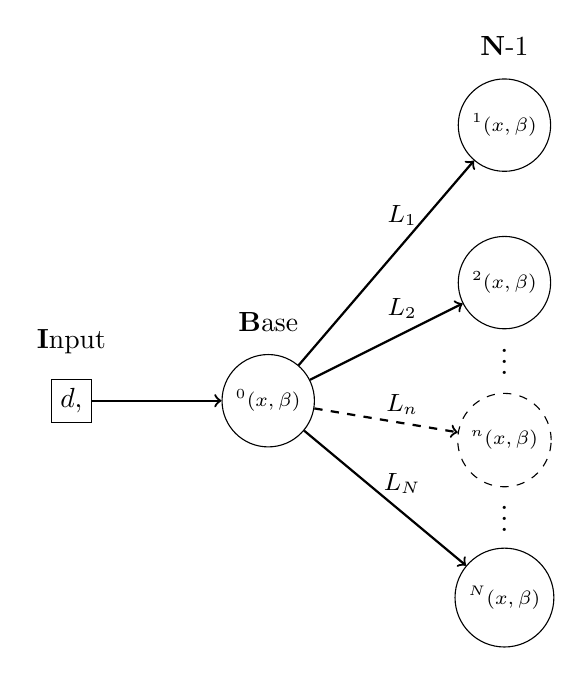
\begin{tikzpicture}

\draw (-2,1.25) node{ \textbf Input };
\draw (-2,.5) node(INPUT)[rectangle,draw]{ $d, \rdelm$};
\draw (.5,1.5) node{ \textbf Base };
\draw (.5,.5) node(ROOT)[circle,draw]{\scriptsize $\ry^0(x,\beta)$ };
\draw (3.5,5) node{ \textbf N-1 };
\draw (3.5,4) node(ONE)[circle,draw]{ \scriptsize $\ry^1(x,\beta)$ };
\draw (3.5,2) node(TWO)[circle,draw]{ \scriptsize $\ry^2(x,\beta)$ };
\draw (3.5,1.1) node(DOTONE){ \large $\vdots$ };
\draw (3.5,0) node(N)[circle,dashed,draw]{ \scriptsize $\ry^n(x,\beta)$ };
\draw (3.5,-.9) node(DOTTWO){ \large $\vdots$ };
\draw (3.5,-2) node(S)[circle,draw]{ \scriptsize $\ry^N(x,\beta)$ };

\draw (2.2,2.85) node(OMG1){ \small $L_1$ };
\draw (2.2,1.67) node(OMG2){ \small $L_2$ };
\draw (2.2,.45) node(OMG){ \small $L_n$ };
\draw (2.2,-.55) node(OMGS){ \small $L_N$ };


\draw[thick, ->] (INPUT) -- (ROOT) ;
\draw[thick, ->] (ROOT) -- (ONE) ;
\draw[thick,->] (ROOT) -- (TWO);
\draw[thick,dashed, ->] (ROOT) -- (N);
\draw[thick,->] (ROOT) -- (S);

%\draw[thick,dashed] (TWO) -- (N);
%\draw[thick,dashed] (N) -- (S);

\end{tikzpicture} 
\caption{N-1 Exogenous Contingencies}
\end{figure}


Reliability standards in power systems include N-1 contingency constraints.  The system must be robust to failures of each individual component due to reasons outside of the control of the system. The branch flows for line $e$ given contingency $n$ can be described with the following relationship
\begin{equation}\label{n1cont}
 \ry_e^n = \ry_e + L_{e n} \ry_n 
\end{equation}
with $L_{en}$ being a line outage factor for outage $n$'s effect on line $e$.  The line outage factor can be found by first finding the branch sensitivity matrix and then applying a scale factor so that when the line outage factor is multiplied by the current branch flow, the response to all other branches is found.
\begin{equation}
L_{en} = \left\{ \begin{array}{c c}
  -1 & \mbox{ if } e=n\\
  A_{en}^B (1-A_{nn}^B)^{-1} & \mbox{ if } A_{nn}^B \neq 1\\
  \mbox{NaN} & \mbox{ o/w }
  \end{array}
\right.
\end{equation}
Shift factors for multiple lines can be found provided certain conditions are met \cite{guler_2007}, however are typically only used for onesmall number of line outages.  A subset of lines will not have line outage factors when $A_{nn}^B = 1$.  In our computational results, we filter out these scenarios for the N-1 analysis.

The mean flow can be found by taking the expecation over the uncertainty in net injections and using equation \ref{n1cont} that describes flow for branch $e$ in contingency $n$.
\begin{equation}
\E{\bD}{\ry_e^n} =  \E{\bD}{\ry_e}  + L_{en} \E{\bD}{\ry_n} 
\end{equation}
We also need to understand the standard deviation of branch flows in the N-1 contingencies in order to form the JCC constraint for each contingency.  Calculating the variance of $\ry_e^n$ and expanding out using equation \ref{n1cont}, we see that the variance of branch flows are
\begin{subequations}
\begin{align}
 Var[\ry_e^n] &= Var[\ry_e] + L^2_{e n} Var[ \ry_n ] + 2 L_{e n} CoVar[ \ry_e, \ry_n ] \\
 &= \pi_e^2 \sD - 2 \pi_e \se + \see \nonumber \\
 &\hspace{30pt} + L_{en}^2 \left[ \pi_n^2 \sD - 2 \pi_n \sn + \snn \right] \nonumber \\
 &\hspace{30pt}+ 2 L_{en} \left[ \pi_{e} \pi_{n} \sD -  \pi_{e} \setwo - \pi_{n} \seone   + \seealone \right]  \\
 &= \left[ \pi_e^2 + 2 L_{en} \pi_e \pi_n + L_{en}^2 \right] \sD \nonumber\\
 &\hspace{30pt} - 2 \left[ \pi_e \se + L_{en} \pi_e \sn + L_{en} \pi_n \se + L_{en}^2 \pi_n \sn \right]  \nonumber \\
&\hspace{30pt} +  \see + 2 L_{en} \sen + L_{en}^2 \snn \\
 &=\psen^2 \sD - 2 \psen \left( \se + L_{en} \sn \right) + \sigma^2_{\psi_{en}}
\end{align}
\end{subequations}
by using equation \ref{covar_branch} for the covariance between two branches and simplifying with shift factor
\begin{equation}
\psen = \pi_e + L_{en} \pi_n
\end{equation}
 which captures the slack distribution response to aggregate demand for branch $e$ in contingency $n$.  It is important to note that not only does the variance depend on the variance of individual line flows, it also depends on the covariance between the line that has failed $n$, and the line we are interested in $e$.  The injection covariance matrix allows you to pre-compute this new parameter $\sigma^2_{\psen}$ which is used in the branch covariance matrix and cutting plane algorithms.
\begin{equation}
\sigma^2_{\psi_{en}} = \sko \skt \left(A_{ek_1} + L_{en} A_{nk_2}\right)^2 \sigot
\end{equation}
The following equations are added to the JCC model \ref{jcc_program} to describe the mean branch flows in the contingencies as well as the standard deviation of branch flows.  Each contingency has seperate line risk variables $z_{en}$ and the system risk is constrained according to that contingencies $\epsilon_n$
\begin{subequations}
\label{jcc_n1_program}
\begin{alignat}{3}
y^+_{en} - y_e - L_{en} y_n & \geq 0 && \forall e,n \label{n1mean2}\\
y^+_{en} + y_e  +  L_{en} y_n & \geq 0 && \forall e,n \label{n1mean2}\\
 s_{en}^2 - \psen^2 \sD + 2 \psen \left( \se + L_{en} \sn \right) &\geq \sigma^2_{\psi_{en}} && \forall e,n \label{n1stddev}\\
z_{en} - g_e(y^+_{en},s_{en}) &\geq 0 && \forall e,n \label{n1linerisk}\\
\sum_e z_{en} &\leq \epsilon_n && \forall n
\end{alignat}
\end{subequations}
Finally, in order to describe the convex, non-analytic risk function for the N-1 contingencies \ref{n1linerisk}, we use the same cutting planes from JCC \ref{line_risk_cuts}.  The cutting planes are calculated at a specific value for slack distribution $\beta$ and the line risk function is underestimated via the gradient.  The cutting planes for the standard deviation of branch flow have changed due to the new covariance calculation taking into account the N-1 contingencies.  These equations are described as follows.
\begin{subequations}
\begin{align}
s_{en} \geq \fenb &+ \sum_j \pfenb \left( \beta_j - \hat{\beta_j} \right)\\
\fenb &= \sqrt{ \psen^2 \sD - 2 \psen \left( \se + L_{en} \sn \right) + \sigma^2_{\psi_{en}}} \\
  \pfenb &= \frac{\left(A_{ej} + L_{en}A_{nj}\right) \left( \psen \sD - \left(\se + L_{en} \sn \right) \right)}{\sqrt{\psen^2 \sD - 2 \psen \left(\se  + L_{en}\sn \right) + \sigma^2_{\psi_{en}} }}
\end{align}
\end{subequations}



\subsection{Random Initial Contingencies for OPA}

\subsubsection{OPA Simulation of Cascading Power Failures}
The fast time scale OPA model (given in chapter one \ref{fast_opa} has been shown to have the same power-law distribution seen in real-world blackout data.  This simulation can be seen as a surrogate model for the response of the power system to rare-event stress.  As such, it is useful to explore the effects different parameters can have and even optimize over them to find any characteristics or trends there may be.

The linear program \ref{dcopf_ow_program} is a load shedding version of the standard DC OPF economic dispatch model.  
\begin{subequations}
\label{dcopf_ow_program}
\begin{alignat}{3}
\min_{\left(x;l,\theta,y\right)} && \displaystyle\sum_j \left[  c_2 x_j^2  + c_1 x_j + c_0 \right] &+ W \sum_i l_i &  \label{jcc_obj}\\
                        && \textstyle \sum_j c^g_{ij} x_j - \sum_j c^b_{ie} y_e   +l_i       &=d_i       && \forall i \label{opf_cons}\\ 
                 && y_e - b_e \textstyle \sum_i c^b_{ie} \theta_i          &=0         && \forall e \label{opf_kcl}\\
                 && l_i &\in \left[ 0, d_i \right] && \forall e \label{opf_loadshed}\\
                 && y_e &\in \left[ -U_e, U_e \right] && \forall e \label{opf_limit}\\
                 && x_j &\in \left[ G^{min}_j, G^{max}_j \right] && \forall j  \label{opf_gen}  
\end{alignat}
\end{subequations}


Let $L$ be the total load shed for a particular dispatch point $x$ and given input $d,\xi,\omega$.
\begin{equation}
L = \sum_i l_i
\end{equation}

\begin{figure}
\centering
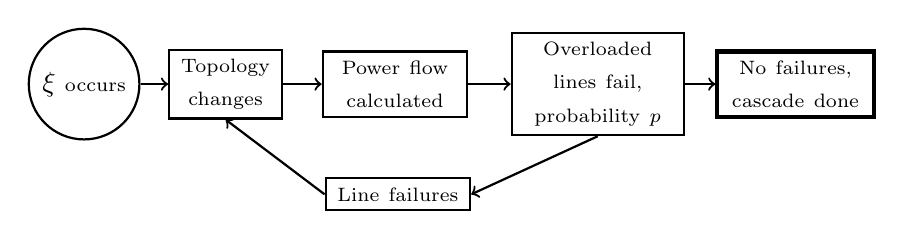
\begin{tikzpicture}
\draw [->,thick] (1,1) node[anchor=east, circle, draw]{$\xi$ \scriptsize occurs}
-- (1.35,1) node(TC)[anchor=west,text width=1.2cm,text centered,  rectangle, draw]{\scriptsize Topology changes};
\draw[->,thick] (TC)
--(3.3,1) node(PF)[anchor=west,text width=1.6cm,text centered, rectangle,draw]{\scriptsize Power flow calculated};
\draw[->,thick] (PF)
--(5.7,1) node(F)[anchor=west,text width=1.95cm, text centered, rectangle, draw]{\scriptsize Overloaded lines fail, probability $p$};
\draw[->,thick] (F)
--(8.3,1) node(DN)[anchor=west,text width=1.75cm, text centered,rectangle,draw,line width=1.5pt]{\scriptsize No failures, cascade done};
\draw[->,thick] (F.south)
--(5.2,-.4) node(LF)[anchor=east,text width=1.6cm, text centered, rectangle, draw]{\scriptsize Line failures };
\draw[->,thick] (LF.west)
-- (TC.south);

\end{tikzpicture} 
\caption{A Review of the OPA short-term cascading process}
\end{figure}
Inputs
\bi
\item $x$, generation
\item $d$, demand
\item $\xi$, initial contingency
\item $\omega$, cascade evolution
\ei

Expected Load Shed
\begin{equation*}
f(x) = \E{\Xi,\Omega}{ \lambda\left(x,d,\xi,\omega\right) }
\end{equation*}


\begin{figure}
\centering
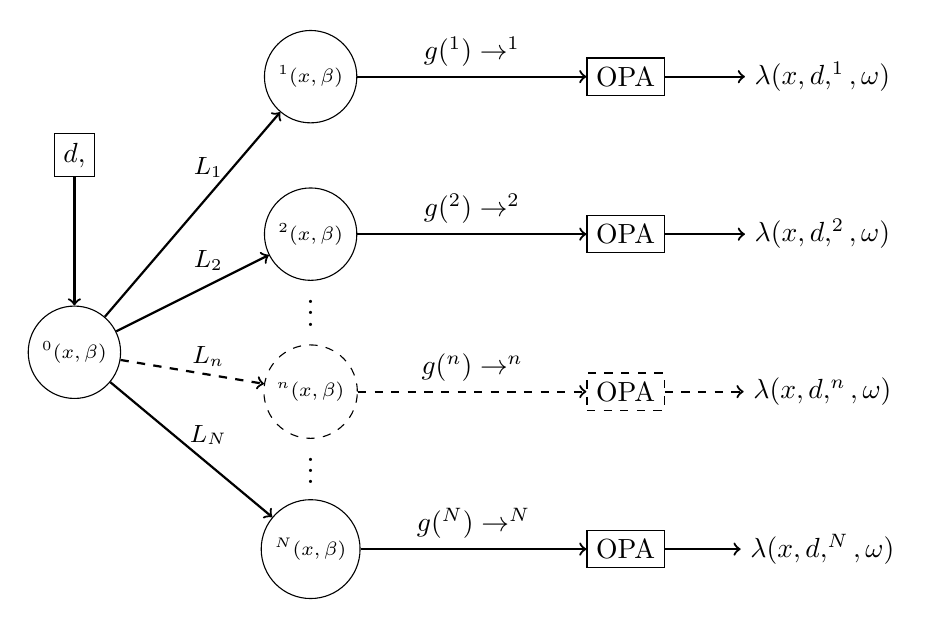
\begin{tikzpicture}

\draw (.5,3) node(INPUT)[rectangle,draw]{ $d, \rdelm$};

\draw (.5,.5) node(ROOT)[circle,draw]{\scriptsize $\ry^0(\alert{x},\alert{\beta})$ };
\draw (3.5,4) node(ONE)[circle,draw]{ \scriptsize $\ry^1(\alert{x},\alert{\beta})$ };
\draw (3.5,2) node(TWO)[circle,draw]{ \scriptsize $\ry^2(\alert{x},\alert{\beta})$ };
\draw (3.5,1.1) node(DOTONE){ \large $\vdots$ };
\draw (3.5,0) node(N)[circle,dashed,draw]{ \scriptsize $\ry^n(\alert{x},\alert{\beta})$ };
\draw (3.5,-.9) node(DOTTWO){ \large $\vdots$ };
\draw (3.5,-2) node(S)[circle,draw]{ \scriptsize $\ry^N(\alert{x},\alert{\beta})$ };

\draw (2.2,2.85) node(OMG1){ \small $L_1$ };
\draw (2.2,1.67) node(OMG2){ \small $L_2$ };
\draw (2.2,.45) node(OMG){ \small $L_n$ };
\draw (2.2,-.55) node(OMGS){ \small $L_N$ };

\draw[thick, ->] (INPUT) -- (ROOT) ;
\draw[thick, ->] (ROOT) -- (ONE) ;
\draw[thick,->] (ROOT) -- (TWO);
\draw[thick,dashed, ->] (ROOT) -- (N);
\draw[thick,->] (ROOT) -- (S);

\draw (7.5,4) node(OPAONE)[rectangle,draw]{ OPA  };
\draw (7.5,2) node(OPATWO)[rectangle,draw]{ OPA  };
\draw (7.5,0) node(OPAN)[rectangle,dashed,draw]{ OPA  };
\draw (7.5,-2) node(OPAS)[rectangle,draw]{ OPA };

\draw[thick, ->] (ONE) -- (OPAONE) node [midway,above] { $g(\ry^1) \rightarrow \rxi^1$ };
\draw[thick,->] (TWO) -- (OPATWO) node [midway,above] { $g(\ry^2) \rightarrow \rxi^2$ };
\draw[thick,dashed, ->] (N) -- (OPAN) node [midway,above] { $g(\ry^n) \rightarrow \rxi^n$ };
\draw[thick,->] (S) -- (OPAS) node [midway,above] { $g(\ry^N) \rightarrow \rxi^N$ };


\draw (10,4) node(ONEFIN)[rectangle]{ $\lambda (x,d,\rxi^1,\omega )$  };
\draw (10,2) node(TWOFIN)[rectangle]{ $\lambda ( x,d,\rxi^2,\omega )$ };
\draw (10,0) node(NFIN)[rectangle,dashed]{ $\lambda ( x,d,\rxi^n,\omega )$ };
\draw (10,-2) node(SFIN)[rectangle]{ $\lambda ( x,d,\rxi^N,\omega)$ };

\draw[thick, ->] (OPAONE) -- (ONEFIN) ;
\draw[thick,->] (OPATWO) -- (TWOFIN);
\draw[thick,dashed, ->] (OPAN) -- (NFIN);
\draw[thick,->] (OPAS) -- (SFIN);


%\draw[thick,dashed] (TWO) -- (N);
%\draw[thick,dashed] (N) -- (S);

\end{tikzpicture}
\caption{JCC N-1 Risk Model to seed random initial contingencies for OPA}
\end{figure}



\begin{algorithm}
\caption{OPA Sampling Algorithm for JCC N-1}\label{opa_sample_alg}
\begin{algorithmic}
\Procedure{OPA}{$x, D, \xi, \omega$}
\State Solve ( \ref{dcopf_program} ) to find base case load shed $z_0$
\State $\xi$ occurs and corresponding changes to the grid are made
\State Stage $s \gets 1$
\While{ Not DONE }
\State Solve ( \ref{dcopf_program} ) to find power injects and branch flows for adjusted grid
\State $\mathbb{O}_s \gets \emptyset$
\For{$\forall e \in \cE $}
\State $\mathbb{O}_s = 
\left\{ 
\begin{array}{lr}
  \mathbb{O}_s + \left\{ e \right\} & \mbox{w/ prob. } h(y_e), \mbox{ draw } \omega_{es} \\
  \mathbb{O}_s & \mbox{o/w }
\end{array}
\right. $ 
\If{ $\mathbb{O}_s \neq \emptyset$ }
\State Modify Grid with $\mathbb{O}_s$
\State $s\gets s+1$
\Else
\State $s^* \gets s,$ calculate $z_{s^*}$, DONE
\EndIf
\EndFor
\EndWhile
\State \label{done}Load Shed $  \lambda\left(x,D,\xi,\omega\right)  = z_{s^*} - z_0$
\EndProcedure
\end{algorithmic}
\end{algorithm}




\begin{figure}
\centering
\begin{tikzpicture}[scale=.9]
\begin{axis}[title=Risk Measure vs Load Shed, xlabel=Load Shed, ylabel={$P \left[ \mbox{At least one line fails} \right]$},legend pos=outer north east]
%,ymax=.04%,xmin=\xmmm,xmax=1,
%	  extra x ticks={.8,.9,.98},
%	  extra x tick style={grid=major},
%	  extra x tick labels={}]


  \addplot+[blue,opacity=.85,only marks, mark size=.35] table[x=LS,y=r] {\mypathojdata/jccS1.out};
  \addlegendentryexpanded{JCC}
  \addplot+[blue,opacity=.85,only marks, mark size=.35] table[x=LS,y=r] {\mypathojdata/jccS2.out};
  \addplot+[blue,opacity=.85,only marks, mark size=.35] table[x=LS,y=r] {\mypathojdata/jccS3.out};
  \addplot+[blue,opacity=.85,only marks, mark size=.35] table[x=LS,y=r] {\mypathojdata/jccS4.out};
  \addplot+[blue,opacity=.85,only marks, mark size=.35] table[x=LS,y=r] {\mypathojdata/jccS5.out};


\end{axis}
\end{tikzpicture}
\caption{Line failure risk and OPA not correlated}
\end{figure}

\subsection{OPA Weighting for JCC}


While it is important that no lines fail, it may be overly restrictive while not actually reducing the risk of large load shedding events, which is the main concern from a system reliability perspective. It would certainly be more beneficial to keep the large high voltage lines in operation that are critical to system stability versus a few small distribution feeders, which may cause some small load shedding but would keep the bad events contained.  In this case, we would like to find the probability of no cascade given an power system operating point.  We can condition this probability on the events of individual lines failing, which we have used previously.


\begin{equation*}
P(\mbox{cascade}|x) = \sum_e P(\mbox{cascade}|e\mbox{ fails}) P(e\mbox{ fails}|x)
\end{equation*}
where $x$ is the operating point and here we worry about the flows $y$ and not the risk from generators.  Let $q_e(y_e) = P(\mbox{cascade}|e\mbox{ fails})$, then we have
\begin{equation} 
H^c(y) = \prod_{e \in \cE} \left( 1 - g_e(y_e)q_e(y_e) \right) \geq 1 - \epsilon
  \end{equation}  
The conditional probabilities $q_e(y_e)$ act as weights on the probability of line failures, so if we set them all to 1 to put an equal importance on every line, we get back our previous formulation.





Want a first order weighting ($\eta$) to approximate OPA
\begin{equation*} 
\sum_e \eta_e \E{\bD}{g(\ry_e^n(\alert{x},\alert{\beta}))} \approx \E{\Xi^n}{\lambda ( \alert{x},d,\rxi^n,\omega) }
\end{equation*}
\begin{equation*}
\eta^T r^n \approx f_n(\alert{x})
\end{equation*}

\begin{equation}\label{jcc_ow_weight}
\sum_e \eta_e r^n_e  \leq \nu_n
\end{equation}

\begin{figure}
\centering
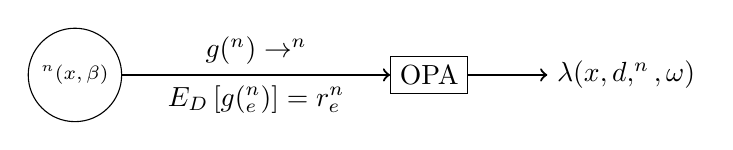
\begin{tikzpicture}
\draw (3.5,4) node(ONE)[circle,draw]{ \scriptsize $\ry^n(\alert{x},\alert{\beta})$ };

\draw (8,4) node(OPAONE)[rectangle,draw]{ OPA  };

\draw[thick, ->] (ONE) -- (OPAONE) node [midway,above] {$g(\ry^n) \rightarrow \rxi^n$ } node[midway,below]{$\E{\bD}{g(\ry_e^n)} = r_e^n$};

\draw (10.5,4) node(ONEFIN)[rectangle]{ $\lambda (\alert{x},d,\rxi^n,\omega )$  };

\draw[thick, ->] (OPAONE) -- (ONEFIN) ;

%\draw<2->[thick,dashed,red] (4.45,3.8) -- (7.2,3.8) -- (7.2,4.8) -- (4.45,4.8) -- (4.45,3.8);
\end{tikzpicture}
\caption{Random initial contingencies and expected failure probabilities}
\end{figure}


\begin{equation*}
\begin{bmatrix}  \alert{r^1_1} & \cdots & \alert{r^1_N} \\ \vdots & \vdots & \vdots \\ \alert{r^N_1} & \cdots & \alert{r^N_N} \end{bmatrix}
\begin{bmatrix} \alert{\eta_1}  \\ \vdots  \\ \alert{\eta_N}  \end{bmatrix} 
=
\begin{bmatrix} \alert{f_1(x)}  \\ \vdots  \\ \alert{f_N(x)}  \end{bmatrix} 
\end{equation*}


\begin{figure}
\centering
\begin{tikzpicture}[scale=1]
\begin{axis}[title=Risk Measure vs Load Shed, xlabel=Load Shed, ylabel=JCC-OW Risk Measure,legend pos=outer north east]
%,ymax=.04%,xmin=\xmmm,xmax=1,
%	  extra x ticks={.8,.9,.98},
%	  extra x tick style={grid=major},
%	  extra x tick labels={}]


  \addplot+[blue,opacity=.85,only marks, mark size=.35] table[x=LS,y=rl] {\mypathojdata/jccS1.out};
  \addlegendentryexpanded{JCC}
  \addplot+[blue,opacity=.85,only marks, mark size=.35] table[x=LS,y=rl] {\mypathojdata/jccS2.out};

  \addplot+[blue,opacity=.85,only marks, mark size=.35] table[x=LS,y=rl] {\mypathojdata/jccS3.out};

  \addplot+[blue,opacity=.85,only marks, mark size=.35] table[x=LS,y=rl] {\mypathojdata/jccS4.out};

  \addplot+[blue,opacity=.85,only marks, mark size=.35] table[x=LS,y=rl] {\mypathojdata/jccS5.out};



\end{axis}
\end{tikzpicture}
\caption{JCC-OW correlated with OPA}
\end{figure}


\subsection{Cutting Plane Algorithm for JCC N-1 with OPA Weighting}
Now, we can describe the cutting plane algorithm for JCC at a high level and give pseudo-code \ref{jcc_alg} for implementation.  The main subproblem the algorithm solves is the standard DC power flow.  After solving, the generator injects $x$, slack distribution $\beta$, and branch flows $y$ are used to calculate risk information about the dispatch point.  To get the risk information, the branch standard deviations $s$ need to be calculated.  With the mean flow $y$ and standard deviation $s$, the line risk $z$ can be calculated.  The sum of line risk is system risk $r$.  If $r$ is less than the required system risk $\epsilon$, the problem is solved.  Otherwise, the algorithm adds cuts for all lines with a positive risk $z$.  The cuts describe how $z$ is related to $y,s$ and how $s$ is related to $\beta$.  Then the power flow subproblem is solved with the addition of the cuts and this repeats until it is infeasible or the risk constraint is satisfied.
\begin{algorithm}
\caption{This cutting plane algorithm solves JCC \ref{jcc_program} with N-1 contingencies\ref{jcc_n1_program} using the OPA weighting scheme \ref{jcc_ow_weight} via linear programs and cutting planes}\label{jcc_ow_alg}
\begin{algorithmic}
\Procedure{JCC}{d,$\Sigma^m$,$\epsilon$,$\epsilon_g$,L,p}
\State $L \gets \emptyset$  (Set of Lines with potential risk)
\State $S \gets \emptyset$  (Set of Cuts)
\State $r \gets 0$ (Risk)
\BState \emph{solve}:
\State $(\hat{x},\hat{\beta},\hat{y}) \gets $Solve DC Power Flow, \cref{jcc_obj,jcc_cons,jcc_kcl,jcc_slack,jcc_limit,jcc_gen1,jcc_gen2}, with cuts $S$, risk $r\leq\epsilon$
\If {Infeasible} \Return Problem Infeasible 
\EndIf
\State Calculate $\hat{s},\hat{z},\hat{r}$ using $(\hat{x},\hat{\beta},\hat{y})$ and \cref{branch_cov,line_risk}
\If {$\hat{r} \leq \epsilon + tol$} \Return Optimal $(\hat{x},\hat{\beta},\hat{y},\hat{s},\hat{z},\hat{r})$
\EndIf
\For{$\forall e$}
\If {$\hat{z_e} \geq tol$}
    \If {$e \notin L$}
            \State $L \gets \left\{L,e\right\}$
            \State Initialize $s_e,z_e$
            \State $r \gets r + z_e$
    \EndIf            
    \State $S \gets$ line risk cuts \ref{line_risk_cuts} for $z_e,y_e,s_e$ dependent on $\hat{z}_e,\hat{y}_e,\hat{s}_e$
    \State $S \gets$ branch variance cuts \ref{branch_var_cuts} for $s_e,\beta_e$ dependent on $\hat{s}_e,\hat{\beta}_e$
\EndIf
\EndFor
\State \textbf{goto} \emph{solve}
\EndProcedure
\end{algorithmic}
\end{algorithm}



\section{Computational Experiments}



\textbf{Higher Cost - Less Rare Event Risk}

\begin{figure}
\centering
\includegraphics[scale=.4]{\mypathoj/histogram-newdes3}
\includegraphics[scale=.4]{\mypathoj/logplot-newdes3}
\caption{Load shed distribution}
\end{figure}


\begin{table}
\centering
Trials \textbf{450400}

\begin{tabular}{|c |  c c | c|}
\hline
Stat & JCC & JCC-OW & diff (\%) \\
\hline
cost&1.78e6 & 1.85e6 & \alert{-3.9} \\
mean&44.0&41.9 & 4.8   \\
num0&199444 & 201984 & 1.3 \\
P95& 138.81& 138.81  &  0         \\
P99& 205.77& 147.12456 &  28.5        \\
P99.8& 441.21& 251.76   &  43      \\
max& 734.29& 612.9      &  16.5            \\
CVaR95 & 182.5 & 155.6 & 14.7 \\
\hline
\end{tabular}
\caption{Rare event risk metrics}
\end{table}


